%%%%%%%%%%%%%%%%%%%%%%%%%%%%%%%%%%%%%%%%%%%%%%%%%%%%%%%%%%%%%%%%%%%
%                                                                 %
%                            APPENDICES                           %
%                                                                 %
%%%%%%%%%%%%%%%%%%%%%%%%%%%%%%%%%%%%%%%%%%%%%%%%%%%%%%%%%%%%%%%%%%%
 
\appendix    % This command is used only once!
%\addcontentsline{toc}{chapter}{APPENDICES}             %toc entry  or:
\addtocontents{toc}{\parindent0pt\vskip12pt APPENDICES} %toc entry, no page #

\chapter{Grounding Semantic Importance Ontology}
Semantic importance (SI) ontology is grounded with the example from the soccer offside detection use case.
The primary incentive to ground the SI ontology is two-fold: to both relate this ontology to a real life use case, and provide details towards understanding and extending the SI ontology.

\begin{figure}[!htbp]
    \centering
    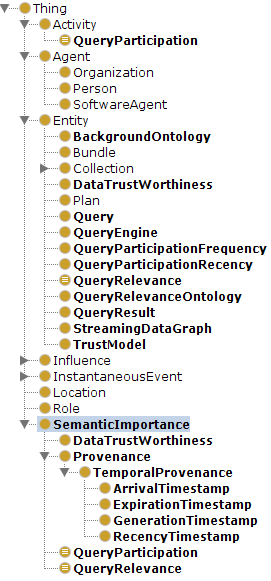
\includegraphics[width=2.5in]{img/app-sio.png}
    \caption{Semantic Importance Ontology Class Hierarchy}
    \label{fig:app-sio}
\end{figure}

%
\section{Class Definition}
As Figure \ref{fig:app-sio} shows, the classes defined in the SI ontology are in bold. 
SI ontology is developed by extending the PROV-O ontology, which is a descriptive ontology. 
As a consequence, the SI ontology can work as a descriptive ontology.
Ontologies are naturally portable, expressive and extendable. 
Thus, SI ontology can be expanded if needed.
With the help of both ontoloy editors (such as Protege\footnote{http://protege.stanford.edu/}) and reasoners, the consistency can be checked to guarantee a valid extension\footnote{https://protegewiki.stanford.edu/wiki/Using\_Reasoners}.

\begin{table}[!htbp]
    \centering
    \caption{SI Ontology Class OWL Definition}
    \begin{tabular}{|c||c|} \hline
         Class Name & Definition  \\ \hhline{|=#=|}
         QueryParticipation & \makecell{(used some QueryEngine) and \\ (used some StreamingDataGraph) and \\(used some BackgroundOntology) and \\(generated some QueryResult)} \\ \hline 
         QueryRelevance & wasDerivedFrom some QueryRelevanceOntology \\ \hline
        %  \multicolumn{2}{|c|}{\makecell{other classes do not need to be defined with OWL since they are not \\compound concepts, and can be defined/described in natural language.}} \\ \hline
    \end{tabular}
    \label{tab:app-socd}
\end{table}

Table \ref{tab:app-socd} shows the class definitions in ontology web language (OWL).
Both \textit{QueryParticipation} and \textit{QueryRelevance} are compound classes, thus needs to be defined in OWL with clear semantics. 
Other classes do not have to be defined in OWL as they can be described in natural language. 
%
\section{Grounded Instances}
This section covers the grounded instances for each class in the SI ontology.
Table \ref{tab:app-gi} shows the example instances for each class. 
The content is the table is self-explanatory, however, I would like to highlight some points that are worth discussion. 

The concept of \textit{DataTrustworthiness} has a concrete instance of \textit{right\_foot\\\_position\_is\_trusted\_left\_foot\_position\_is\_untrusted}.
In Chapter 5 where soccer offside use case is evaluated, it has been mentioned that \textit{Player\_B4}'s sensor has failed.
This observation leads me to propose this simple data trustworthiness model, which essentially only trusts left foot position. 
This might be trivial, but the point is that \textit{DataTrustworthiness}, if deployed, should have a trust model that can either be an equation or a ontology. 

The instance of \textit{Query} is \textit{who\_commits\_an\_offside\_offence}. 
When deployed in the system, this is actually a physical continuous query file that can be loaded in the system. 
\textit{QueryEngine} indicates what triple store and SPARQL query engine that the system use. 
In my case, I used Stardog. 
Nonetheless, any other database will be the instance of \textit{QueryEngine} if used. 

\textit{QueryParticipationFrequency} describes how many times the data participates in the query during its valid time period.
When deployed in the system, it is actually an integer value that can be used to rank the data. 

\textit{StreamingDataGraph} class describes the actual RDF streaming data.
In my case, I encapsulate each triple in a unique graph, which makes it easier to process the data.
In fact, a graph can contain multiple streaming data items. 
An example would be to use the streaming source as the graph ID and all the generated data items are within this graph. 

\begin{center}
\begin{longtable}{|c||c||c|}
\caption[SI Ontology Grounded Instances]{SI Ontology Grounded Instances} \label{tab:app-gi} \\

\hline \multicolumn{1}{|c||}{\textbf{Class Name}} & \multicolumn{1}{c||}{\textbf{Instance Example}} & \multicolumn{1}{c|}{\textbf{Annotation}} \\ \hhline{|=#=#=|}
\endfirsthead

\multicolumn{3}{c}%
{{\bfseries \tablename\ \thetable{} -- continued from previous page}} \\
\hline \multicolumn{1}{|c||}{\textbf{Class Name}} &
\multicolumn{1}{c||}{\textbf{Instance Example}} &
\multicolumn{1}{c|}{\textbf{Annotation}} \\ \hline 
\endhead

\hline \multicolumn{3}{|r|}{{Continued on next page}} \\ \hline
\endfoot

\hline
\endlastfoot
\makecell{Background\\Ontology} & \makecell{soccer\_offside\_\\background\_ontology} & \makecell{soccer offside background \\ ontology provide necessary \\ knowledge for defining \\\& determing soccer offside.} \\ \hline
\makecell{DataTrust-\\worthiness} & \makecell{right\_foot\_position\_\\is\_trusted\_\\left\_foot\_position\_\\is\_untrusted} & \makecell{right foot position is\\ trusted, left foot position \\is not trusted} \\ \hline
Query & \makecell{who\_commits\_an\_\\offside\_offence} & \makecell{the query ``who commits an offside \\offence'' is the target query and \\registered in the system} \\ \hline
QueryEngine & \makecell{stardog\_triplestore\_\\SPARQL\_engine} & \makecell{in soccer offside use case, Stardog \\triplestore is used thus its SPARQL \\query engine is used.} \\ \hline
\makecell{Query\\Participation\\Frequency} & \makecell{graph1\_query\_\\participation\_\\frequency\_value} & \makecell{graph1 refers to\\``graph1\_PlayerA\_a\_Attacker''\\ (see StreamingDataGraph \\individuals for details)} \\ \hline
\makecell{Query\\Participation\\Recency} & \makecell{graph1\_query\_\\participation\_\\recency\_timestamp} & \makecell{the timestamp when graph1 \\participates in the query.} \\ \hline
\makecell{Query\\Relevance\\Ontology} & \makecell{soccer\_offside\_query\_\\relevance\_ontology} & \makecell{the query relevance ontology to \\help filter irrelevant data out} \\ \hline
\makecell{QueryResult} & \makecell{PlayerA\_commits\_\\an\_offside\_offence} & \makecell{the query result indicates \\that PlayerA commits \\an offside offence} \\ \hline
\makecell{Streaming\\DataGraph} & \makecell{graph1\_PlayerA\_a\_\\Attacker.\\graph2\_PlayerA\_a\_\\BallLastToucher.\\graph3\_PlayerA\_a\_\\PlayerAtOffsidePosition.\\graph4\_PlayerB\_a\_\\Attacker.} & \makecell{``graph1\_PlayerA\_a\_Attacker'' \\indicates that the triple \\``PlayerA a Attacker''\\ is in graph1. In this example, \\every graph only has 1 triple. \\(It could have more, \\but we set it to only have 1)} \\ \hline
TrustModel & \makecell{left\_foot\_position\_\\has\_trust\_score\_\\of\_1\_right\_has\_0} & \makecell{trust model stamps \\trust scores to data} \\ \hline
\makecell{Arrival\\Timestamp} & \makecell{graph1\_arrival\_\\timestamp} & \makecell{the arrival timestamp of graph1} \\ \hline
\makecell{Expiration\\Timestamp} & \makecell{graph1\_expiration\_\\timestamp} & \makecell{the expiration timestamp \\of graph1} \\ \hline
\makecell{Generation\\Timestamp} & \makecell{graph1\_generation\_\\timestamp} & \makecell{the generation timestamp \\of graph1} \\ \hline
\makecell{Recency\\timestamp} & \makecell{graph1\_query\_\\participation\_recency\_\\timestamp} & \makecell{the most recent query \\participation timestamp \\of graph1} \\ \hline
\makecell{Query\\Participation} & \makecell{graph1\_graph2\_graph3\_\\background\_ontology\_\\stardog\_query\_engine\_\\target\_query\_\\query\_result} & \makecell{please refer to Table \ref{tab:app-socd}} \\ \hline
\makecell{Query\\Relevance} & \makecell{graph1\_is\_relevant\_\\to\_query\\graph7\_is\_irrelevant\_\\to\_query} & \makecell{the relevance is determined \\by the query relevance ontology} \\
\end{longtable}
\end{center}
%
\section{Instance Property Assertions}
Instances are inter-related.
This relationship is established via properties. 

\begin{center}
\begin{longtable}{|c||c||c|}
\caption[SI Ontology Instance Property Assertions]{SI Ontology Instance Property Assertions} \label{tab:app-ipa} \\

\hline \multicolumn{1}{|c||}{\textbf{Class Name}} & \multicolumn{1}{c||}{\textbf{Instance Example}} & \multicolumn{1}{c|}{\textbf{Property Assertion}} \\ \hhline{|=#=#=|}
\endfirsthead

\multicolumn{3}{c}%
{{\bfseries \tablename\ \thetable{} -- continued from previous page}} \\
\hline \multicolumn{1}{|c||}{\textbf{Class Name}} &
\multicolumn{1}{c||}{\textbf{Instance Example}} &
\multicolumn{1}{c|}{\textbf{Property Assertion}} \\ \hline 
\endhead

\hline \multicolumn{3}{|r|}{{Continued on next page}} \\ \hline
\endfoot

\hline
\endlastfoot
\makecell{DataTrust-\\worthiness} & \makecell{left\_foot\_position\_\\is\_trusted\_\\right\_foot\_position\_\\is\_untrusted} & \makecell{object property assertion: \\wasDerivedFrom \\ left\_foot\_position\_\\has\_trust\_score\_\\of\_1\_right\_has\_0\\ data property assertion: \\value 10} \\ \hline
\makecell{Query\\Participation\\Frequency} & \makecell{graph1\_query\_\\participation\_\\frequency\_value} & \makecell{data property assertion: \\value 3} \\ \hline
\makecell{Query\\Participation\\Recency} & \makecell{graph1\_query\_\\participation\_\\recency\_timestamp} & \makecell{data property assertion: \\value ``2011-07-16T02:52:02Z''\\\string^\string^dateTime } \\ \hline
\makecell{Arrival\\Timestamp} & \makecell{graph1\_arrival\_\\timestamp} & \makecell{data property assertion: \\value ``2011-08-16T02:52:02Z''\\\string^\string^dateTime } \\ \hline
\makecell{Expiration\\Timestamp} & \makecell{graph1\_expiration\_\\timestamp} & \makecell{data property assertion: \\value ``2011-09-16T02:52:02Z''\\\string^\string^dateTime } \\ \hline
\makecell{Generation\\Timestamp} & \makecell{graph1\_generation\_\\timestamp} & \makecell{data property assertion: \\value ``2011-10-16T02:52:02Z''\\\string^\string^dateTime } \\ \hline
\makecell{Recency\\timestamp} & \makecell{graph1\_query\_\\participation\_recency\_\\timestamp} & \makecell{data property assertion: \\value ``2011-11-16T02:52:02Z''\\\string^\string^dateTime } \\ \hline
\makecell{Query\\Participation} & \makecell{graph1\_graph2\_graph3\_\\background\_ontology\_\\stardog\_query\_engine\_\\target\_query\_\\query\_result} & \makecell{object property assertion: \\generated PlayerA\_commits\_an\_\\offside\_offence; \\used graph1\_PlayerA\_\\a\_attacker; \\used stardog\_triplestore\_\\sparql\_engine; \\generated graph1\_query\_\\participation\_frequency\_\\value; \\generated graph1\_query\_\\participation\_recency\_\\timestamp; \\used soccer\_offside\_\\background\_ontology; \\used graph2\_PlayerA\_\\a\_BallLastToucher; \\used graph3\_PlayerA\_\\a\_PlayerAtOffsidePosition} \\ \hline
\makecell{Query\\Relevance} & \makecell{graph1\_is\_relevant\_\\to\_query\\graph7\_is\_irrelevant\_\\to\_query} & \makecell{object property assertion: \\ wasDerivedFrom soccer\_offside\_query\_\\relevance\_ontology} \\
\end{longtable}
\end{center}
%
\section{Described Examples}
This section shows some concrete examples for selected classes and instances. 
\subsection{Query Participation Example}
Data items participate in a query if they contain necessary information used by the query engine to return non-empty answers.
When a data item particpates in a query, related meta-data such as the timestamp and frequency value can be collected. 
Consider a snapshot of streaming data as follows:

\begin{lstlisting}[caption={Example Streaming Data}, label={lst:app-esd}]
PlayerA a Attacker, graph1
PlayerA a BallLastToucher, graph2
PlayerA a PlayerAtOffsidePosition, graph3
PlayerB a Attacker, graph4
PlayerB hasPosition LeftFootPosition, graph5
PlayerB hasPosition RightFootPosition, graph6
PlayerC a Defender, graph7
\end{lstlisting}

In this use case, I used stardog SPARQL engine as the \textit{QueryEngine}, the \textit{BackgroundOntology} encodes that a player who commits an offside offence should be: (i) player a Attacker, (ii) player a BallLastToucher, and (iii) player a PlayerAtOffsidePosition.
For the streaming data in Listing A.1, graph1 contains Triple i, graph2 contains Triple ii, graph3 contains Triple iii, graph4 contains Triple i, graph5 doesn’t convey Triple i, ii, or iii, graph6 doesn’t convey Triple i, ii, or iii, graph7 doesn’t convey Triple i, ii, or iii.
Thus, a \textit{QueryResult} is given: Player A commits an offside offence. 
According to QueryParticipation class definition,  ``used some QueryEngine) and (used some StreamingDataGraph) and (used some BackgroundOntology) and (generated some QueryResult)'', 
the streaming data graphs that are used to generate the query result is said to have participated in the query. 
Thus: graph1, graph2, \& graph3 have successfully participated in the query, while graph4, graph5, graph6, \& graph7 have unsuccessfully participated in the query.

Graph1, graph2, \& graph3's frequencies and recency will be updated.
Graph4, graph5, graph6, \& graph7’s frequencies and recency won’t be updated. 
If ranked by query participation, then graph1, graph2, graph3 will rank equally on the top, and graph4, graph5, graph6, graph7 will rank equally at the bottom.

%
\section{Semantic Importance Ontology File}
The following shows the full file of the SI ontology.
The source file is also available at the github repository\footnote{https://github.com/raymondino/SemanticImportanceOntology}.
\lstset{
basicstyle=\ttfamily,
  columns=fullflexible,
  keepspaces=true,
    frame=single,
    breaklines=true,
    postbreak=\raisebox{0ex}[0ex][0ex]{\ensuremath{\color{red}\hookrightarrow\space}}
}
\begin{lstlisting}[language=XML,caption={Semantic Importance Ontology File (update this file)}]
<?xml version="1.0"?>
<!DOCTYPE rdf:RDF [
    <!ENTITY prov "http://www.w3.org/ns/prov#" >
    <!ENTITY owl "http://www.w3.org/2002/07/owl#" >
    <!ENTITY xsd "http://www.w3.org/2001/XMLSchema#" >
    <!ENTITY rdfs "http://www.w3.org/2000/01/rdf-schema#" >
    <!ENTITY rdf "http://www.w3.org/1999/02/22-rdf-syntax-ns#" >
]>
<rdf:RDF xmlns="http://www.semanticweb.org/rui/ontologies/semanticimportance#"
     xml:base="http://www.semanticweb.org/rui/ontologies/semanticimportance"
     xmlns:rdfs="http://www.w3.org/2000/01/rdf-schema#"
     xmlns:prov="http://www.w3.org/ns/prov#"
     xmlns:owl="http://www.w3.org/2002/07/owl#"
     xmlns:xsd="http://www.w3.org/2001/XMLSchema#"
     xmlns:rdf="http://www.w3.org/1999/02/22-rdf-syntax-ns#">
    <owl:Ontology rdf:about="http://www.semanticweb.org/rui/ontologies/semanticimportance">
        <owl:versionIRI rdf:resource="http://www.semanticweb.org/rui/ontologies/semanticimportance/1.0"/>
        <owl:imports rdf:resource="http://www.w3.org/ns/prov-o#"/>
    </owl:Ontology>
    
    <!-- Object Properties -->
    
    <!-- http://www.semanticweb.org/rui/ontologies/semanticimportance#isRelevantTo -->

    <owl:ObjectProperty rdf:about="http://www.semanticweb.org/rui/ontologies/semanticimportance#isRelevantTo">
        <rdfs:comment>describes how relevant A is to B. The relevance can be described with a relevance ontology</rdfs:comment>
    </owl:ObjectProperty>
    
    <!-- Classes -->
    
    <!-- http://www.semanticweb.org/rui/ontologies/semanticimportance#ArrivalTimestamp -->

    <owl:Class rdf:about="http://www.semanticweb.org/rui/ontologies/semanticimportance#ArrivalTimestamp">
        <rdfs:subClassOf rdf:resource="http://www.semanticweb.org/rui/ontologies/semanticimportance#TemporalProvenance"/>
    </owl:Class>

    <!-- http://www.semanticweb.org/rui/ontologies/semanticimportance#DataGraph -->

    <owl:Class rdf:about="http://www.semanticweb.org/rui/ontologies/semanticimportance#DataGraph">
        <rdfs:subClassOf rdf:resource="&prov;Entity"/>
    </owl:Class>
    
    <!-- http://www.semanticweb.org/rui/ontologies/semanticimportance#DataTrustWorthiness -->

    <owl:Class rdf:about="http://www.semanticweb.org/rui/ontologies/semanticimportance#DataTrustWorthiness">
        <rdfs:subClassOf rdf:resource="http://www.semanticweb.org/rui/ontologies/semanticimportance#SemanticImportance"/>
        <rdfs:subClassOf rdf:resource="&prov;Entity"/>
    </owl:Class>

    <!-- http://www.semanticweb.org/rui/ontologies/semanticimportance#ExpirationTimestamp -->

    <owl:Class rdf:about="http://www.semanticweb.org/rui/ontologies/semanticimportance#ExpirationTimestamp">
        <rdfs:subClassOf rdf:resource="http://www.semanticweb.org/rui/ontologies/semanticimportance#TemporalProvenance"/>
    </owl:Class>

    <!-- http://www.semanticweb.org/rui/ontologies/semanticimportance#GenerationTimestamp -->

    <owl:Class rdf:about="http://www.semanticweb.org/rui/ontologies/semanticimportance#GenerationTimestamp">
        <rdfs:subClassOf rdf:resource="http://www.semanticweb.org/rui/ontologies/semanticimportance#TemporalProvenance"/>
    </owl:Class>

    <!-- http://www.semanticweb.org/rui/ontologies/semanticimportance#Provenance -->

    <owl:Class rdf:about="http://www.semanticweb.org/rui/ontologies/semanticimportance#Provenance">
        <rdfs:subClassOf rdf:resource="http://www.semanticweb.org/rui/ontologies/semanticimportance#SemanticImportance"/>
    </owl:Class>

    <!-- http://www.semanticweb.org/rui/ontologies/semanticimportance#Query -->

    <owl:Class rdf:about="http://www.semanticweb.org/rui/ontologies/semanticimportance#Query">
        <rdfs:subClassOf rdf:resource="&prov;Entity"/>
    </owl:Class>

    <!-- http://www.semanticweb.org/rui/ontologies/semanticimportance#QueryEngine -->

    <owl:Class rdf:about="http://www.semanticweb.org/rui/ontologies/semanticimportance#QueryEngine">
        <rdfs:subClassOf rdf:resource="&prov;Entity"/>
    </owl:Class>

    <!-- http://www.semanticweb.org/rui/ontologies/semanticimportance#QueryParticipation -->

    <owl:Class rdf:about="http://www.semanticweb.org/rui/ontologies/semanticimportance#QueryParticipation">
        <owl:equivalentClass>
            <owl:Class>
                <owl:intersectionOf rdf:parseType="Collection">
                    <owl:Restriction>
                        <owl:onProperty rdf:resource="&prov;generated"/>
                        <owl:someValuesFrom rdf:resource="http://www.semanticweb.org/rui/ontologies/semanticimportance#QueryResult"/>
                    </owl:Restriction>
                    <owl:Restriction>
                        <owl:onProperty rdf:resource="&prov;used"/>
                        <owl:someValuesFrom rdf:resource="http://www.semanticweb.org/rui/ontologies/semanticimportance#DataGraph"/>
                    </owl:Restriction>
                    <owl:Restriction>
                        <owl:onProperty rdf:resource="&prov;used"/>
                        <owl:someValuesFrom rdf:resource="http://www.semanticweb.org/rui/ontologies/semanticimportance#QueryEngine"/>
                    </owl:Restriction>
                </owl:intersectionOf>
            </owl:Class>
        </owl:equivalentClass>
        <rdfs:subClassOf rdf:resource="http://www.semanticweb.org/rui/ontologies/semanticimportance#SemanticImportance"/>
        <rdfs:subClassOf rdf:resource="&prov;Activity"/>
    </owl:Class>
  
    <!-- http://www.semanticweb.org/rui/ontologies/semanticimportance#QueryParticipationFrequency -->

    <owl:Class rdf:about="http://www.semanticweb.org/rui/ontologies/semanticimportance#QueryParticipationFrequency">
        <rdfs:subClassOf rdf:resource="&prov;Entity"/>
    </owl:Class>

    <!-- http://www.semanticweb.org/rui/ontologies/semanticimportance#QueryParticipationRecency -->

    <owl:Class rdf:about="http://www.semanticweb.org/rui/ontologies/semanticimportance#QueryParticipationRecency">
        <rdfs:subClassOf rdf:resource="&prov;Entity"/>
    </owl:Class>

    <!-- http://www.semanticweb.org/rui/ontologies/semanticimportance#QueryRelevance -->

    <owl:Class rdf:about="http://www.semanticweb.org/rui/ontologies/semanticimportance#QueryRelevance">
        <owl:equivalentClass>
            <owl:Class>
                <owl:intersectionOf rdf:parseType="Collection">
                    <owl:Restriction>
                        <owl:onProperty rdf:resource="&prov;hadPrimarySource"/>
                        <owl:someValuesFrom>
                            <owl:Restriction>
                                <owl:onProperty rdf:resource="http://www.semanticweb.org/rui/ontologies/semanticimportance#isRelevantTo"/>
                                <owl:someValuesFrom rdf:resource="http://www.semanticweb.org/rui/ontologies/semanticimportance#Query"/>
                            </owl:Restriction>
                        </owl:someValuesFrom>
                    </owl:Restriction>
                    <owl:Restriction>
                        <owl:onProperty rdf:resource="&prov;wasDerivedFrom"/>
                        <owl:someValuesFrom rdf:resource="http://www.semanticweb.org/rui/ontologies/semanticimportance#QueryRelevanceOntology"/>
                    </owl:Restriction>
                </owl:intersectionOf>
            </owl:Class>
        </owl:equivalentClass>
        <rdfs:subClassOf rdf:resource="http://www.semanticweb.org/rui/ontologies/semanticimportance#QueryParticipationRecency"/>
        <rdfs:subClassOf rdf:resource="http://www.semanticweb.org/rui/ontologies/semanticimportance#SemanticImportance"/>
    </owl:Class>

    <!-- http://www.semanticweb.org/rui/ontologies/semanticimportance#QueryRelevanceOntology -->

    <owl:Class rdf:about="http://www.semanticweb.org/rui/ontologies/semanticimportance#QueryRelevanceOntology">
        <rdfs:subClassOf rdf:resource="&prov;Entity"/>
    </owl:Class>

    <!-- http://www.semanticweb.org/rui/ontologies/semanticimportance#QueryResult -->

    <owl:Class rdf:about="http://www.semanticweb.org/rui/ontologies/semanticimportance#QueryResult">
        <rdfs:subClassOf rdf:resource="&prov;Entity"/>
    </owl:Class>

    <!-- http://www.semanticweb.org/rui/ontologies/semanticimportance#RecencyTimestamp -->

    <owl:Class rdf:about="http://www.semanticweb.org/rui/ontologies/semanticimportance#RecencyTimestamp">
        <rdfs:subClassOf rdf:resource="http://www.semanticweb.org/rui/ontologies/semanticimportance#TemporalProvenance"/>
    </owl:Class>

    <!-- http://www.semanticweb.org/rui/ontologies/semanticimportance#SemanticImportance -->

    <owl:Class rdf:about="http://www.semanticweb.org/rui/ontologies/semanticimportance#SemanticImportance"/>

    <!-- http://www.semanticweb.org/rui/ontologies/semanticimportance#TemporalProvenance -->

    <owl:Class rdf:about="http://www.semanticweb.org/rui/ontologies/semanticimportance#TemporalProvenance">
        <rdfs:subClassOf rdf:resource="http://www.semanticweb.org/rui/ontologies/semanticimportance#Provenance"/>
    </owl:Class>

    <!-- http://www.semanticweb.org/rui/ontologies/semanticimportance#TrustModel -->

    <owl:Class rdf:about="http://www.semanticweb.org/rui/ontologies/semanticimportance#TrustModel">
        <rdfs:subClassOf rdf:resource="&prov;Entity"/>
    </owl:Class>

    <!-- Individuals -->

    <!-- http://www.semanticweb.org/rui/ontologies/semanticimportance#aDataGraph -->

    <owl:NamedIndividual rdf:about="http://www.semanticweb.org/rui/ontologies/semanticimportance#aDataGraph">
        <rdf:type rdf:resource="http://www.semanticweb.org/rui/ontologies/semanticimportance#DataGraph"/>
        <isRelevantTo rdf:resource="http://www.semanticweb.org/rui/ontologies/semanticimportance#aTargetQuery"/>
    </owl:NamedIndividual>

    <!-- http://www.semanticweb.org/rui/ontologies/semanticimportance#aDataItemIsUsedByQueryEngineForResults -->

    <owl:NamedIndividual rdf:about="http://www.semanticweb.org/rui/ontologies/semanticimportance#aDataItemIsUsedByQueryEngineForResults">
        <prov:used rdf:resource="http://www.semanticweb.org/rui/ontologies/semanticimportance#aDataGraph"/>
        <prov:generated rdf:resource="http://www.semanticweb.org/rui/ontologies/semanticimportance#aQueryResult"/>
        <prov:used rdf:resource="http://www.semanticweb.org/rui/ontologies/semanticimportance#stardogQueryEngine"/>
    </owl:NamedIndividual>

    <!-- http://www.semanticweb.org/rui/ontologies/semanticimportance#aQueryResult -->

    <owl:NamedIndividual rdf:about="http://www.semanticweb.org/rui/ontologies/semanticimportance#aQueryResult">
        <rdf:type rdf:resource="http://www.semanticweb.org/rui/ontologies/semanticimportance#QueryResult"/>
    </owl:NamedIndividual>

    <!-- http://www.semanticweb.org/rui/ontologies/semanticimportance#aSoccerOffsideRelevanceOntology -->

    <owl:NamedIndividual rdf:about="http://www.semanticweb.org/rui/ontologies/semanticimportance#aSoccerOffsideRelevanceOntology">
        <rdf:type rdf:resource="http://www.semanticweb.org/rui/ontologies/semanticimportance#QueryRelevanceOntology"/>
    </owl:NamedIndividual>

    <!-- http://www.semanticweb.org/rui/ontologies/semanticimportance#aTargetQuery -->

    <owl:NamedIndividual rdf:about="http://www.semanticweb.org/rui/ontologies/semanticimportance#aTargetQuery">
        <rdf:type rdf:resource="http://www.semanticweb.org/rui/ontologies/semanticimportance#Query"/>
    </owl:NamedIndividual>

    <!-- http://www.semanticweb.org/rui/ontologies/semanticimportance#aTimestampOfRecentQueryParticipation -->

    <owl:NamedIndividual rdf:about="http://www.semanticweb.org/rui/ontologies/semanticimportance#aTimestampOfRecentQueryParticipation">
        <rdf:type rdf:resource="http://www.semanticweb.org/rui/ontologies/semanticimportance#RecencyTimestamp"/>
        <prov:value rdf:datatype="&xsd;dateTime">2011-07-16T02:52:02Z</prov:value>
    </owl:NamedIndividual>
 
    <!-- http://www.semanticweb.org/rui/ontologies/semanticimportance#aTimestampWhenDataArrives -->

    <owl:NamedIndividual rdf:about="http://www.semanticweb.org/rui/ontologies/semanticimportance#aTimestampWhenDataArrives">
        <rdf:type rdf:resource="http://www.semanticweb.org/rui/ontologies/semanticimportance#ArrivalTimestamp"/>
        <prov:value rdf:datatype="&xsd;dateTime">2011-07-16T02:52:02Z</prov:value>
    </owl:NamedIndividual>

    <!-- http://www.semanticweb.org/rui/ontologies/semanticimportance#aTimestampWhenDataExpires -->

    <owl:NamedIndividual rdf:about="http://www.semanticweb.org/rui/ontologies/semanticimportance#aTimestampWhenDataExpires">
        <rdf:type rdf:resource="http://www.semanticweb.org/rui/ontologies/semanticimportance#ExpirationTimestamp"/>
        <prov:value rdf:datatype="&xsd;dateTime">2011-07-16T02:52:02Z</prov:value>
    </owl:NamedIndividual>

    <!-- http://www.semanticweb.org/rui/ontologies/semanticimportance#aTimestampWhenDataIsGenerated -->

    <owl:NamedIndividual rdf:about="http://www.semanticweb.org/rui/ontologies/semanticimportance#aTimestampWhenDataIsGenerated">
        <rdf:type rdf:resource="http://www.semanticweb.org/rui/ontologies/semanticimportance#GenerationTimestamp"/>
        <prov:value rdf:datatype="&xsd;dateTime">2011-07-16T02:52:02Z</prov:value>
    </owl:NamedIndividual>

    <!-- http://www.semanticweb.org/rui/ontologies/semanticimportance#aTrustEquation -->

    <owl:NamedIndividual rdf:about="http://www.semanticweb.org/rui/ontologies/semanticimportance#aTrustEquation">
        <rdf:type rdf:resource="http://www.semanticweb.org/rui/ontologies/semanticimportance#TrustModel"/>
    </owl:NamedIndividual>

    <!-- http://www.semanticweb.org/rui/ontologies/semanticimportance#dataItemXisRelevantToQueryY -->

    <owl:NamedIndividual rdf:about="http://www.semanticweb.org/rui/ontologies/semanticimportance#dataItemXisRelevantToQueryY">
        <prov:value rdf:datatype="&xsd;boolean">true</prov:value>
        <prov:hadPrimarySource rdf:resource="http://www.semanticweb.org/rui/ontologies/semanticimportance#aDataGraph"/>
        <prov:wasDerivedFrom rdf:resource="http://www.semanticweb.org/rui/ontologies/semanticimportance#aSoccerOffsideRelevanceOntology"/>
    </owl:NamedIndividual>

    <!-- http://www.semanticweb.org/rui/ontologies/semanticimportance#stardogQueryEngine -->

    <owl:NamedIndividual rdf:about="http://www.semanticweb.org/rui/ontologies/semanticimportance#stardogQueryEngine">
        <rdf:type rdf:resource="http://www.semanticweb.org/rui/ontologies/semanticimportance#QueryEngine"/>
    </owl:NamedIndividual>
 
    <!-- http://www.semanticweb.org/rui/ontologies/semanticimportance#theTimestampWhenQueryEngineUsesADataItemToProduceResult -->

    <owl:NamedIndividual rdf:about="http://www.semanticweb.org/rui/ontologies/semanticimportance#theTimestampWhenQueryEngineUsesADataItemToProduceResult">
        <rdf:type rdf:resource="http://www.semanticweb.org/rui/ontologies/semanticimportance#QueryParticipationRecency"/>
        <prov:generatedAtTime rdf:datatype="&xsd;dateTime">2011-07-16T02:52:02Z</prov:generatedAtTime>
        <prov:wasGeneratedBy rdf:resource="http://www.semanticweb.org/rui/ontologies/semanticimportance#aDataItemIsUsedByQueryEngineForResults"/>
    </owl:NamedIndividual>

    <!-- http://www.semanticweb.org/rui/ontologies/semanticimportance#theTotalTimesOfADataItemUsedByQueryEngineForResults -->

    <owl:NamedIndividual rdf:about="http://www.semanticweb.org/rui/ontologies/semanticimportance#theTotalTimesOfADataItemUsedByQueryEngineForResults">
        <rdf:type rdf:resource="http://www.semanticweb.org/rui/ontologies/semanticimportance#QueryParticipationFrequency"/>
        <prov:value rdf:datatype="&xsd;integer">3</prov:value>
        <prov:wasGeneratedBy rdf:resource="http://www.semanticweb.org/rui/ontologies/semanticimportance#aDataItemIsUsedByQueryEngineForResults"/>
    </owl:NamedIndividual>
    
    <!-- http://www.semanticweb.org/rui/ontologies/semanticimportance#trustworthinessInstance -->

    <owl:NamedIndividual rdf:about="http://www.semanticweb.org/rui/ontologies/semanticimportance#trustworthinessInstance">
        <rdf:type rdf:resource="http://www.semanticweb.org/rui/ontologies/semanticimportance#DataTrustWorthiness"/>
        <prov:value rdf:datatype="&xsd;integer">10</prov:value>
        <prov:wasDerivedFrom rdf:resource="http://www.semanticweb.org/rui/ontologies/semanticimportance#aTrustEquation"/>
    </owl:NamedIndividual>
</rdf:RDF>
\end{lstlisting}
%